\documentclass{article}

\newcommand{\question}[2]{{\noindent \bf #1} #2}
\usepackage[french]{babel}
\usepackage{hyperref}
\usepackage{amsmath}
\usepackage{verbatim}
\usepackage{shortvrb}
\ifpdf \usepackage[pdftex]{graphicx} \pdfcompresslevel=9

\title{TP Unity: \\ Cin\'ematique inverse avec l'algorithme CCD }
\date{\today}
\author{Steve Tonneau\\ IRISA}

\begin{document}
\maketitle

\section*{Introduction}
Ce TP propose de traiter un probl\`eme concret, r\'ecurent dans le domaine de l'animation, celui de la 
cin\'ematique inverse. La partie \ref{problem} de ce document est consacr\'ee \`a la description du probl\`eme. Aussi
les lecteurs les plus \'eclair\'es pourront directement passer \`a la partie \ref{implementation}. Cette seconde partie a pour 
but de guider les \'etudiants dans l'impl\'ementation de l'algorithme CCD (pour Cyclic Coordinate Descent), tr\`es utilis\'e,
en particulier dans le domaine du jeu vid\'eo, pour r\'esoudre le probl\`eme de cin\'ematique inverse.
On l'impl\'ementera d'abord en 2, puis en 3 dimensions.

\subsection*{Public concern\'e}
Ce tp s'adresse \`a des \'etudiants en premi\`ere ann\'ee d'informatique. Il requiert une connaissance
minimale du moteur Unity 3d \footnote{\href{http://unity3d.com/unity}{http://unity3d.com/unity.}} (Menus, syst\`eme de scripts).
Les signatures des m\'ethodes utilis\'ees sont pr\'esent\'ees en C\#, mais il est facile de les transposer pour les langages Boo et javascript
\'egalement accept\'es sous Unity. Aussi il est \'egalement n\'ecessaire d'avoir des connaissances dans un de ces langages cibles.

Pour comprendre et impl\'ementer l'algorithme CCD sous Unity, des connaissances math\'ematiques de niveau lyc\'ee sont n\'ecessaires.

\subsection*{Dur\'ee}
TODO 

\subsection*{Mat\'eriel}
Un squelette de projet est disponible \`a l'adresse TODO. Il n\'ecessite une version d'Unity (gratuite ou pro) sup\'erieure ou \'egale \`a la version 4.1. \\

Le projet comprend:
\begin{itemize}
	\item Une sc\`ene CCD.scene. Elle comprend elle-m\^eme:
		\begin{itemize} 
			\item Une hi\'erarchie de sph\`eres qui servira de cha\^ine cin\'ematique pour l'exercice;
			\item Un cube §Target§, qui repr\'esentera la cible \`a atteindre par notre cha\^ine cin\'ematique.
		\end{itemize}
	\item Un squelette de script §CCD.cs§, qu'il va falloir modifier.
\end{itemize}

\section{Probl\'ematique: La cin\'ematique inverse}
\label{problem}

\subsection{Exemple introductif: r\'eglage de l'heure}
\label{montreex}
Consid\'erons la montre \`a gauche de la figure \ref{watch}:
\begin{figure}[htb]
  \centering
    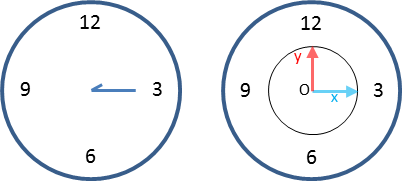
\includegraphics[]{watch2}
  \caption{
          \textit{A gauche: Une montre indiquant 2h15. A droite: la m\^eme montre munie d'un rep\`ere cart\'esien (Ox, Oy).}}
		   \label{watch}
\end{figure}

\subsubsection*{Cin\'ematique directe}
Nous munissons notre montre d'un rep\`ere cart\'esien \textit{(Ox, Oy)} (figure \ref{watch}, droite), dans lequel la longueur
de la grande aiguille vaut 1.
Nous appelons l'extr\'emit\'e ext\'erieure de l'aiguille \textbf{effecteur}. On observe en fait que l'effecteur se d\'eplace
le long du cercle trigonom\`etrique associ\'e au rep\`ere \textit{(Ox, Oy)}. \\
Ce d\'eplacement est r\'ealis\'e par une rotation d'un angle $\theta$ autour d'un troisi\'eme axe $Oz = Ox \wedge Oy$.

On d\'efinit donc la fonction \textit{f}, telle que
 \begin{displaymath}  
f(\theta) =  \begin{pmatrix}
cos(\theta) \\
sin(\theta)
\end{pmatrix}
 \end{displaymath}
avec \begin{math} \theta \in [0, 2\pi[ \end{math}. \\

Gr\^ace \`a $f$ on peut conna\^itre la position de l'effecteur de la grande aiguille en fonction de l'angle $\theta$. Par exemple, si $\theta = -\pi / 2$,
l'effecteur est \`a la position $\begin{pmatrix}
0 \\
-1
\end{pmatrix}$, comme montr\'e sur la figure \ref{2h30}

\begin{figure}[htb]
  \centering
    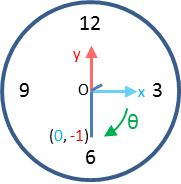
\includegraphics[]{watchrotcart}
  \caption{
          \textit{Si on choisit $\theta = -\pi / 2$, la montre indique maintenant 2h30.}}
		   \label{2h30}
\end{figure}

Ceci constitue un exemple de \textbf{cin\'ematique directe}: \`a partir d'un angle $\theta$, nous calculons une position
$\begin{pmatrix} x \\ y \end{pmatrix}$.

\subsubsection*{Cin\'ematique inverse}
On consid\`ere le probl\`eme inverse:
On souhaite r\'egler l'heure \`a 2h30,  c'est \`a dire que l'extr\'emit\'e de la grande aiguille ait pour coordonn\'ees $\begin{pmatrix} 0 \\ -1 \end{pmatrix}$.
Quelle valeur doit prendre l'angle $\theta$ pour atteindre cet objectif? \\

On d\'efinit la fonction $f^{-1}$, telle que
 \begin{displaymath}  
f^{-1}(x, y) =  acos(x) * sgn(y)
 \end{displaymath}
avec $sgn(y) =  -1$ si $y < 0$, $sgn(y) =  1$ sinon. \\

$f^{-1}$ permet de calculer l'angle $\theta$ n\'ecessaire \`a l'atteinte de la position $\begin{pmatrix} x \\ y \end{pmatrix}$.
Ceci est un exemple de \textbf{cin\'ematique inverse}.

\subsection{Cin\'ematique en deux dimensions}
\subsubsection*{D\'efinition d'une cha\^ine cin\'ematique}
Pour ce tp, nous d\'efinissons une cha\^ine cin\'ematique comme un ensemble $n$ de barres rigides $c_i, i = 0,1, ... , n-1$ 
maintenues deux \`a deux ensemble \`a leurs extr\^emit\'es par des articulations $q_i$.
L'articulation $q_j, j = 1, ... , n-1$ connecte les barres $c_j-1$ et $c_j$. $q_0$
connecte la premi\`ere barre et l'environnement. Cette articulation est appel\'ee racine.
La derni\`ere barre n'est connect\`ee qu'\`a une de ses extr\'emit\'es; on appelle l'extr\'emit\'e libre \textbf{effecteur} $e$.

Par exemple la grande aiguille de la montre pr\'esent\'ee (figure 
\ref{watchcine}) est une cha\^ine compos\'ee d'une seule barre rigide, qui comprend donc la racine
et l'effecteur. \\

Un angle $\theta_i$ qui d\'ecrit la rotation associ\'ee \`a une articulation $q_i$, comme le montre 
la figure \ref{chainangle}.


\begin{figure}[htb]
  \centering
    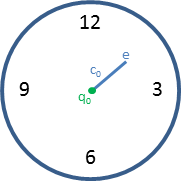
\includegraphics[]{watchcine}
  \caption{
          \textit{La grande aiguille de la montre est une cha\^ine cin\'ematique compos\'ee d'une seule barre rigide.}}
		   \label{watchcine}
\end{figure}

\begin{figure}[htb]
  \centering
    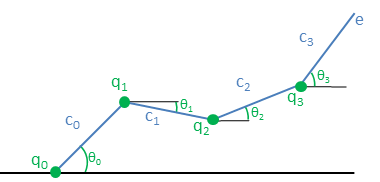
\includegraphics[]{chainangles}
  \caption{
          \textit{Une chaine cin\'ematique compos\'ee de quatre corps rigides.}}
		   \label{chainangle}
\end{figure}

\subsubsection*{Cin\'ematique directe}
Dans un probl\`eme de cin\'ematique directe, on cherche \`a d\'eterminer la position de l'effecteur $e$ en fonction
des valeurs d'angles $\theta_i$ de la cha\^ine cin\'ematique.

On veut donc trouver la fonction $f$ telle que:

\begin{displaymath}  
f\begin{pmatrix} \theta_0 \\ ... \\ \theta_{n-1} \end{pmatrix} = \begin{pmatrix}
x_e \\
y_e
\end{pmatrix}
\end{displaymath}
 
 \subsubsection*{Cin\'ematique inverse}
Dans un probl\`eme de cin\'ematique inverse, on cherche \`a d\'eterminer une combinaison de valeurs d'angles $\theta_i$ qui permette
d'atteindre la position $\begin{pmatrix} x_e \\ y_e \end{pmatrix}$.

On veut donc trouver la fonction $f^{-1}$ telle que:

\begin{displaymath}  
f^{-1} \begin{pmatrix} x_e \\ y_e \end{pmatrix} =  \begin{pmatrix} \theta_0 \\ ... \\ \theta_{n-1} \end{pmatrix}
 \end{displaymath}
 
 Le probl\`eme est que, dans les cas complexes, f n'est pas bijective:
 \begin{itemize}
 \item elle n'est pas surjective car $f^{-1}$ n'est pas forc\'ement d\'efinie partout (figure \ref{outareach});
 \item elle n'est pas injective car il peut exister plusieurs solutions qui permettent d'atteindre la position
 $\begin{pmatrix} x_e \\ y_e \end{pmatrix}$(figure \ref{multisol}).
 \end{itemize}
 
 
 \begin{figure}[htb]
  \centering
    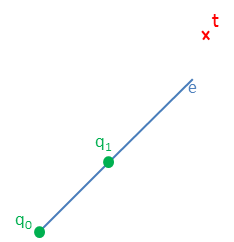
\includegraphics[]{outareach}
  \caption{
          \textit{Le point $t$ ne peut \^etre atteint par l'effecteur $e$.}}
		   \label{outareach}
\end{figure}
 
 
 \begin{figure}[htb]
  \centering
    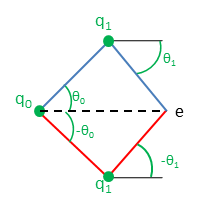
\includegraphics[]{multisol}
  \caption{
          \textit{Diff\'erentes combinaisons d'angles peuvent aboutir \`a la m\^eme position pour l'effecteur $e$.}}
		   \label{multisol}
\end{figure}

Quand une cha\^ine cin\'ematique est trop complexe, il est difficile, voire impossible de d\'efinir correctement $f^{-1}$; c'est pour
cela que des m\'ethodes num\'eriques ont \'et\'e mises au point pour calculer les valeurs de $f^{-1}$, comme la m\'ethode CCD.
  
\subsection{Cin\'ematique en 3 dimensions}
Nous avons vu qu'en deux dimensions nous consid\'erons des rotations autour de l'axe $Oz = Ox \wedge Oy$.
En 3 dimensions, il nous faudra \'egalement consid\'erer des rotations autour des axes Ox et Oy (figure \ref{rot3d}).
 
  \begin{figure}[htb]
  \centering
    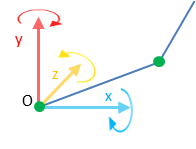
\includegraphics[]{rot3d}
  \caption{
          \textit{Articulation en 3 dimensions: 3 rotations sont possibles.}}
		   \label{rot3d}
\end{figure}
 
\section{Impl\'ementation de l'algorithme CCD}
\label{implementation}
 
\end{document}